\vspace{-2em}

\section{Introduction}

Partial differential equations (PDEs) are differential equations which contain a-priori unkown multivariable functions and their partial derivatives. They are used to model various physical phenomena, such as heat, fluid dynamics or quantum mechanics. There are several numerical methods to solve PDEs. A common one is the finite-difference method (FDM), which approaches the differential equation by discretizing the problem space and converting the PDE to a system of linear equations. The obtained linear system can be solved using an iterative procedure which updates the solution until convergence is reached.

The original paper proposes to use machine learning techniques in order to find high performing update rules instead of designing them by hand \cite{original_paper}, while still guaranteeing convergence.  
In order to fulfill these requirements the learned solver is an adapted existing standard solver, from which the convergence property is inherited by enforcing that a fixed point of the original solver is a fixed point for the trained solver as well. We stress that the goal is not to find a new solver, but to optimize an existing one. To be precise the learned part operates with the residuals after applying the standard solver. This construction allows application to other existing linear iterative solvers of equivalent design.

Since a linear iterative solver can be expressed as a product of convolutional operations, it is not far fetched to use the similar techniques used in deep learning in order to find such an optimal operator.
In order to test this approach a solver was trained to solve a 2D Poisson equation on a square-shaped geometry with Dirichlet boundary conditions. This solver is then tested on larger geometries of two shapes and different boundary values. No significant loss of performance was observed; generalization is thus reached.

For more information we kindly refer to the original paper \cite{original_paper}.

\section{Background}

In this section, we give a short introduction to the Poisson problem and iterative solvers, which will help to understand the justification of using a convolutional neural network to obtain a solver.

\subsection{Poisson Equation}

The Poisson equation is a second order linear partial differential equation (PDE). In order to guarantee the existence and uniqueness of a solution, appropriate boundary conditions needs to be prescribed [\cite{elliptic}]. In this paper only Dirichlet boundary conditions were considered.
The Poisson problem hence reads:
\begin{equation}
Find \quad u \colon \overline{\Omega}=\Omega\cup\partial\Omega \to \sR \quad s.t
\begin{cases}
\nabla^2 u = \sum_{i}\frac{\partial^2}{\partial x_i^2} = f(\vx) & in \ \Omega\\
u = b(\vx) & on \ \partial \Omega\\
\end{cases}
\label{poisson_def}
\end{equation}
Where $\Omega \subset \sR^k$ is a bounded domain with boundary $\partial\Omega$. More specifically we consider $\overline{\Omega} = [0,1]^2$.

\subsection{Finite Difference Method}
In order to solve complex, real-world PDEs a numerical approach must be used, as analytic solutions can be seldom found. As a first step the problem is discretized by transforming the solution space from $u\colon\sR^k \to \sR$ to $u_h\colon\sD^k \to \sR$, where $\sD^k$ is a discrete subset of $\sR^k$. In this paper $k = 2$ and denoting by $N$ the domain size, we introduce a regular grid $\overline{\Omega}_h \subset \sD^k$ on  $\overline{\Omega}$: 

\begin{align*}
\overline{\Omega}_h &= \{\vx_{i,j} = (ih, jh) \qquad i,j = 0,...,N-1 \} \\
{\Omega}_h &= \{\vx_{i,j} = (ih, jh) \qquad i,j = 1,...,N-2 \} \\
\partial\Omega_h &= \overline{\Omega}_h \setminus {\Omega}_h
\end{align*}
with $h=1/(N-1)$ and denoting by ${\Omega}_h$ the interior points, and by $\partial\Omega_h$ the boundary points.
Equation \ref{poisson_def} can be approximated as follows, discretizing and approximating $\nabla^2$:
\begin{equation}
Find \quad u_h \colon \overline{\Omega}_h \to \sR \quad s.t.
\begin{cases}
\frac{1}{h^2}(u_{i-1,j} + u_{i+1,j} + u_{i,j-1} + u_{i,j+1} - 4u_{i,j})=f_{i,j} & in \ \Omega_h \\
u_{i,j} = b_{i,j} & in \ \partial\Omega_h \\
\end{cases}
\label{Eq:discrete}
\end{equation}

It can be shown that the discrete approximation in equation \ref{Eq:discrete} is stable and that $||u-u_h||_{L^2}\leq c h^2$ with $c$ being a constant (\cite{finitedif}).
Introducing a matrix $\mA \in \sR^{N^2\times N^2}$ and a vector $\vf\in \sR^{N^2}$ problem definition \ref{Eq:discrete} can be written as a linear system: 
\begin{equation}
    \mA \vu = \vf
    \label{Eq:system}
\end{equation}

With $\mA$ being a pentadiagonal matrix:

\begin{equation*}
\emA_{i, j} = 
\begin{cases}
    1       & \quad \text{if } i = j, \\
    -\frac{1}{4} & \quad \text{else if } j \in \{i \pm 1, i \pm N\}, \\
    0       & \quad \text{else}
\end{cases}    
\end{equation*}

and defining $i^{\star}=\floor{i/N}$, $j^{\star}=(i\mod N)$ we have:
\begin{align*}
    \evf_i = \frac{h^2}{4}f(\vx_{i^{\star},j^{\star}})
\end{align*}

In order to prescribe the boundary conditions we introduce a reset operator $\mathcal{G}$:

\begin{equation*}
    \mathcal{G}(\vu, \vb) = \mG \vu + (\mI-\mG)\vb
\end{equation*}

where $\mG \in \sR^{N^2\times N^2}$ is a diagonal matrix and $\vb \in \sR^{N^2}$ is the boundary values vector:

\begin{align*}
    \emG_{i,i} &= 1, \quad \evb_{i} = 0 \quad \; \quad \;\;\;\quad \quad \vx_{i^{\star},j^{\star}}\in \Omega_h \\
    \emG_{i,i} &= 0, \quad \evb_{i} = b(\vx_{i^{\star},j^{\star}})  \qquad \vx_{i^{\star},j^{\star}}\in \partial\Omega_h
\end{align*}

We note that the proposed approach to enforce boundary conditions is restricted to iterative methods solving linear systems equivalent to equation \ref{Eq:system}.
Moreover we have not investigated how this approach can be generalized to other type of boundary conditions other than Dirichlet or to different iterative methods such as the Gauss-Seidel method.

\subsection{Iterative Solvers}
A linear iterative solver finds the solution of a linear system by iteratively updating an initial solution guess $\vu^0$.
The updating step can be expressed as:

\begin{equation*}
\vu^{k+1} = \mT\vu^k + \vc
\end{equation*}

Where $\mT$ is a constant update matrix and $\vc$ is a constant vector.
A common approach to build $\mT$ and $\vc$ is to split $\mA$ into $\mA = \mM-\mN$ and by rewriting $\mA\vu=\vf$ as $\mM\vu=\mN\vu + \vf$ the following updating rule naturally arises:
\begin{equation*}
\vu^{k+1} = \mM^{-1}\mN\vu^k + \mM^{-1}\vf
\end{equation*}
For more details we refer readers to \cite{leveque} or to \cite{original_paper}.

\subsubsection{Jacobi method}
Setting $\mM = diag(\mA)$ leads to the so called Jacobi method. In the case of the Poisson problem $\mM=\mI$ and $\mT=\mI-\mA$, hence relying on the previously introduced reset operator the Jacobi method reads:
\begin{align*}
\vu^{k+1} &= \Psi(\vu^k)\\
          &= \mathcal{G}((\mI-\mA)\vu^k + \vf, \vb)\\
          &= \mG((\mI-\mA)\vu^k + \vf) + (\mI-\mG)\vb\\
          &= \mG((\mI-\mA)\vu^k + \vf-\vb) + \vb
\label{jacobiMatrix}
\end{align*}

The Jacobi method can also be implemented by convolution and point-wise operations, as we explain in the following. We define by $\omega_J \ast \underline{\vu}$ the 2D convolution with zero padding of the kernel $\omega_J$ and $\underline{\vu} \in \sR^{N\times N}$, with:
\begin{align*}
\omega_{J} = \left (
 \begin{smallmatrix}
0 & 1/4 & 0 \\
1/4 & 0 & 1/4 \\
0 & 1/4 & 0
\end{smallmatrix}
\right )
\end{align*}

We can also define a new reset operator $\underline{\mathcal{G}}$ denoting by $\circ$ the Hadamard product:

\begin{equation*}
    \underline{\mathcal{G}}(\underline{\vu}, \underline{\vb}) = \underline{\mG} \circ \underline{\vu} + \underline{\vb}
\end{equation*}

where $\underline{\mG},\underline{\vb} \in \sR^{N\times N}$:
\begin{align*}
    \underline{\emG}_{i,j} &= 1, \quad \underline{\evb}_{i,j} = 0 \quad \; \quad  \qquad \vx_{i,j}\in \Omega_h \\
    \underline{\emG}_{i,j} &= 0, \quad \underline{\evb}_{i,j} = b(\vx_{i,j})  \qquad \vx_{i,j}\in \partial\Omega_h
\end{align*}

Finally the Jacobi method can be written as 
\begin{align*}
\underline{\vu}^{k+1} &= \underline{\Psi}(\underline{\vu}^k)\\
                      &=\underline{\mathcal{G}}(\omega_J \ast \underline{\vu}^k + \underline{\vf}, \underline{\vb})\\
                      &= \underline{\mG}\circ(\omega_J \ast \underline{\vu}^k + \underline{\vf}) + \underline{\vb}
\end{align*}

\section{Learning Process}

We want to find an operator $\mathcal{H}$ to optimize the convergence of the Jacobi method for the Poisson problem of the form:
\begin{align*}
\underline{\vu}^{k+1} &=  \underline{\Phi}_{\mathcal{H}}(\vu^k) \\            &=\underline{\Psi}(\underline{\vu}^k) + \mathcal{H}(\underline{\Psi}(\underline{\vu}^k)-\underline{\vu}^k)
\end{align*}
We define $\mathcal{H}$ as the composition of $K$ operations:
\begin{align*}
    \mathcal{H}(\underline{\vw}) &= \mathcal{H}_K...(\mathcal{H}_3(\mathcal{H}_2(\mathcal{H}_1(\underline{\vw}))))...)\\
    \mathcal{H}_i(\underline{\vw}) &= \underline{\mG} \circ (\omega_i \ast \underline{\vw})
\end{align*}
As in the Jacobi method $\omega_i \ast \underline{\vw}$ represents a 2D convolution with zero padding and no bias term of a $3\times3$ kernel $\omega_i$ with $\underline{\vw}$. The operation with $\underline{\mG}$ ensures that the residuals are always zero at the boundary points.

\subsection{Interpretation of $\mathcal{H}$ }
The operator $\mathcal{H}$ can also be expressed as a matrix vector multiplication. We call $\mH \in \sR^{N^2 \times N^2}$ the equivalent matrix:

\begin{equation*}
    \mH = \mG\mH_K\mG\mH_{K-1}...\mG\mH_1
\end{equation*}

$\mH_i$ is a banded matrix which is obtained from the corresponding $3\times3$ kernel $\omega_i$ as follows:

\begin{alignat*}{3}
\emH_{i,i-N-1}  & = \omega_{0,0}  &\qquad \emH_{i,i-N} &  = \omega_{0,1}  &\qquad \emH_{i,i-N+1}  & = \omega_{0,2}\\
\emH_{i,i-1}  & = \omega_{1,0}  &  \emH_{i,i} & = \omega_{1,1} &  \emH_{i,i+1}  & = \omega_{1,2}\\
\emH_{i,i+N-1}  & = \omega_{2,0}  &  \emH_{i,i+N}  & = \omega_{2,1}  &  \emH_{i,i+N+1}  & = \omega_{2,2}
\end{alignat*}

So the new method can be written using only matrix multiplications as:

\begin{align*}
\vu^{k+1} &= \Phi_{\mH}(\vu^k) = \Psi(\vu^k) + \mH(\Psi(\vu^k)-\vu^k)\\
\label{jacobiMatrix}
\end{align*}
This interpretation is useful because if the following holds:
\begin{equation}
    \rho(\mG\mT+\mH(\mG\mT-\mI)) < 1
    \label{Eq:spectral}
\end{equation}
then the method is guaranteed to convergence to a fixed point. Which can be used during training time to enforce the convergence requirement.

\section{Training and Generalization}
\subsection{Training}
In order to find the optimal operator $\mathcal{H}$ the corresponding linear neural network is created. Each 2D convolutional layer has a kernel size $3\times 3$ and zero bias, without any activation function. The training phase is done on a set of Poisson problem instances $\mathcal{D}$. A problem instance is uniquely defined by $\underline{\mG}$, $\underline{\vf}$, and $\underline{\vb}$.
We set $\vf=\bold{0}$ and we use a square domain with a $16\times16$ grid. Each side exhibits a different but constant boundary value chosen from a uniform distribution on the interval [-1, 1]. For each problem instance the error between the ground truth solution $\underline{\vu} ^ {\star}(\underline{\mG}, \underline{\vf}, \underline{\vb})$ and the computed solution using $\underline{\Phi}_{\mathcal{H}}$ with $k$ iterations contributes to the loss function. The ground truth solution is obtained using the Jacobi method operator $\underline{\Psi}$ with a sufficiently high number of iterations $k=2000$.
The optimization objective is then defined as:

%In order to find the optimal operation $\mH(\vu)$ a linear deep neural network of multiple convolutional layers with kernel size 3 and without any bias terms or activation function is created, trained on a small grid with a square boundary, e.g. a $16\times16$ grid, and tested on larger grids and different boundary shapes. 


\begin{align}
    \underset{\mathcal{H}}{\text{min}} \sum_{\underline{\mG},\underline{\vb},\underline{\vf} \in \mathcal{D}; k \in \mathcal{DU}(1, 20)} \left \Vert \underline{\Phi}_{\mathcal{H}}^k (\underline{\vu}^0, \underline{\mG}, \underline{\vf}, \underline{\vb}) - \underline{\vu} ^ {\star}(\underline{\mG}, \underline{\vf}, \underline{\vb}) \right \Vert _2 ^ 2
\end{align}

With $k \in \mathcal{DU}(1, 20)$ we denote the sampling of k from a discrete uniform distribution on the interval $[1, 20]$. The initial guess $\underline{\vu}^0$ is sampled from a Gaussian distribution: $\underline{\vu}^0 \sim \mathcal{N}(0, 1)$. We have not enforced the any constraint to guarantee that the obtained operator $\underline{\Phi}_{\mathcal{H}}$ converges to a fixed point. Since it is not possible to express analytically the spectral radius in Inequality \ref{Eq:spectral} it is not clear how a regularization term could be added to the objective function.
A possible solution would be to check the spectral radius at each iteration and if $>1$ under-relax the weights of the convolutional kernels $\omega_i$.
However this technique is highly computationally expensive since it requires to compute the eigenvalues of a $N^2\times N^2$ matrix at each iteration. 
We showed however that empirically, without explicitly enforcing this constraint, the optimization yields an operator $\underline{\Phi}_{\mathcal{H}}$ which indeed converges for the tested problems.



\subsubsection{Optimizer}
We are using Adadelta as the optimizer of our model, because of its ability to adapt over time and its minimal computational overhead. The method requires no manual adjustment of a learning rate and is robust to various selection of hyperparameters. Adadelta adjusts the learning rate by slowing down learning around a local optima, when the accuracy changes by a small margin. Adadelta also uses the idea of momentum to accelerate progress along dimensions in which the gradient consistently point in the same direction. This idea is implemented by keeping track of the previous parameter update and applying an exponential decay with a decay factor of $\rho = 0.9$ (\cite{adadelta_ref}). \\

\begin{table}[h]
\centering
\caption{Parameters used in the training process.}
\begin{tabular}{| c | c |}
	%\rowcolor{gray!50}
	  \hline
      Grid size $N\times N$  & $16\times 16$ \\
      \hline
      Number of problems $|\mathcal{D}|$  & 50 \\
      \hline
      Batch size $|\mathcal{B}|$ & 10  \\
      \hline
      Max epochs & 1000 \\
      \hline
      Tolerance &  1e-6  \\
      \hline
      Optimizer  & Adadelta   \\
      \hline
      $\rho$ & 0.9  \\
      \hline
\end{tabular}
\label{table:parameters}
\end{table}

The training was done with \textit{batch optimization} of size $|\mathcal{B}|=10$.
At each epoch the set of problem instances $\mathcal{D}$ is randomly split in $\ceil{|\mathcal{D}|/|\mathcal{B}|}$ subsets.
The loss for these batches is defined as the sum over all losses in the batch. The pseudo code for our training process is given in Algorithm 1.

\begin{algorithm}[h]
    \SetKwData{Us}{$u^*$}
    \SetKwFunction{Solver}{Solver}
    \SetKwFunction{ConvNet}{ConvNetSolver}
    \SetKwInOut{Parameter}{Parameter}
    \SetKwInOut{Data}{Data}
    \SetKwInOut{Output}{Result}
    \Parameter{ConvNet $\mathcal{H}$}
    \Data{$\underline{\mG}$,$\underline{\vb}$,$\underline{\vf}$}
    \Output{Optimal ConvNet $\mathcal{H}$}
    \BlankLine
    \For{ $ \{\underline{\mG}, \underline{\vf}, \underline{\vb} \} \in D $ }{
    Compute $\underline{\vu} ^ {\star}(\underline{\mG}, \underline{\vf}, \underline{\vb})$\\
    Randomly sample $k_i$ from $\mathcal{DU}(1, 20)$\\
    Sample $\underline{\vu}^0$ from a Gaussian with $\mu =0 $ and $\sigma = 1$}
    \Repeat{$\Vert loss_{epoch - 1} - loss_{epoch} \Vert$ < $Tolerance$}{
    $\mathcal{D^{\star}}$ $\leftarrow$ \text{randomly split $\mathcal{D}$ in $\ceil{|\mathcal{D}|/|\mathcal{B}|}$ subsets} \\
    \For{$\mathcal{B} \in \mathcal{D^{\star}}$}{
    $loss_{batch} \leftarrow \sum_{p \in \mathcal{B}} \left \Vert \underline{\Phi}_{\mathcal{H}}^k(p) - \underline{\vu} ^ {\star}(p) \right \Vert_2^2$ \\
    Compute the gradient of the loss function \\
    Update weights of $\mathcal{H}$}
    $loss_{epoch} \leftarrow \sum_{p \in \mathcal{D}} \left \Vert \underline{\Phi}_{\mathcal{H}}^k(p) - \underline{\vu}^{\star}(p) \right \Vert_2^2$
    }
 \label{training}
 \caption{Training Process}
\end{algorithm}

\subsection{Hyper Parameter Search}
In order to find the optimal number of layers and learning rate a simple grid search is performed.
As a first step we fix the number of layers $K=3$ and compare the loss evolution for different learning rates $\gamma$.
From Figure \ref{fig:hyperparam_learning_rate} it is evident the the loss decay is highly dependent on the choice of the learning rate. For $\gamma$ small the loss tends to converge to what probably is a local minimum while for high values it can lead to divergence problems; note that in Figure \ref{fig:hyperparam_learning_rate} the loss for $\gamma=1e-4$ is not displayed since the optimization diverged. 

%\begin{figure}[]
%    \centering
%    \begin{minipage}{.5\textwidth}
%        \centering
%        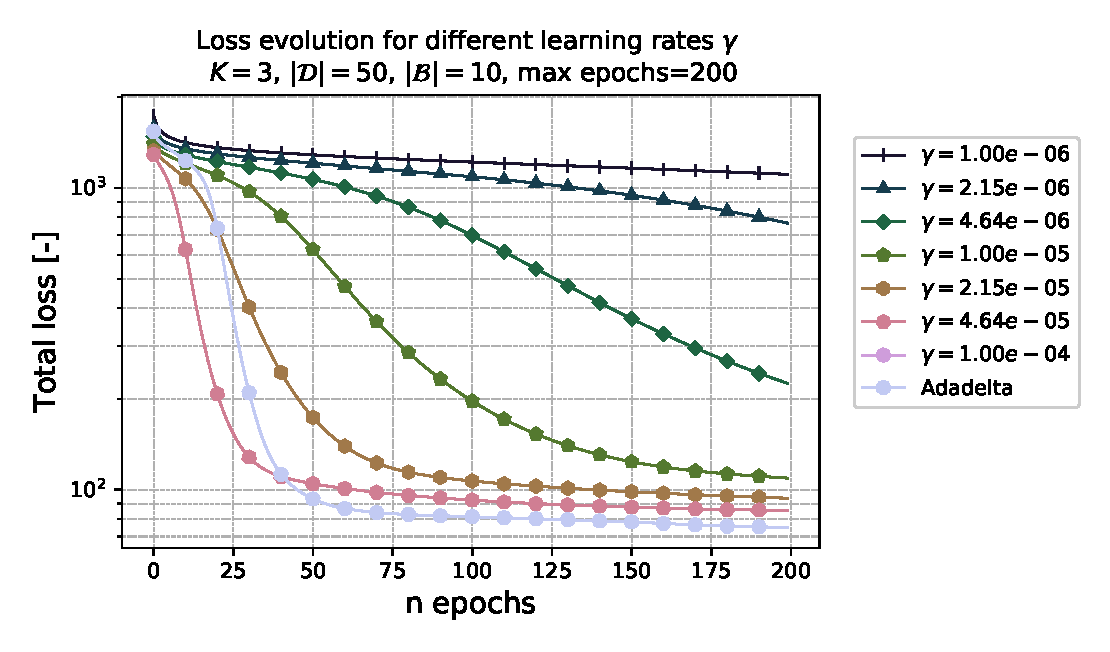
\includegraphics[width=\linewidth]{figs/hyper.eps}
%    \end{minipage}%
%    \begin{minipage}{0.5\textwidth}
%        \centering
%        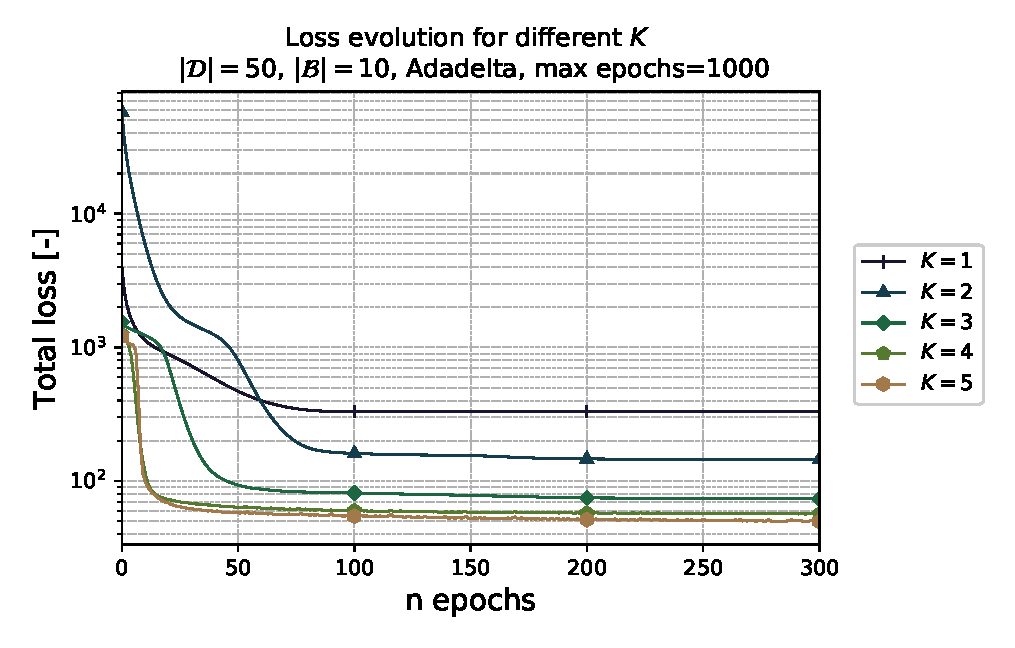
\includegraphics[width=\linewidth]{figs/comparison_K.eps}
%    \end{minipage}
%    \caption{Example solutions for the two domains.}
%    \label{fig:example_solutions}
%\end{figure}


\begin{figure}[h]
\centering
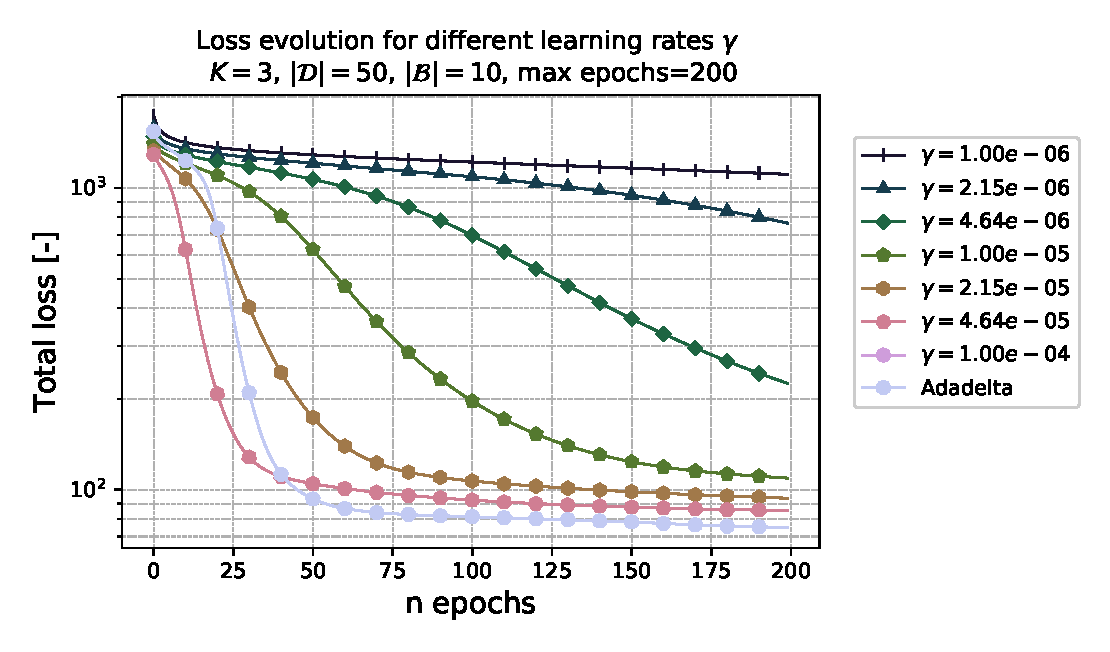
\includegraphics[width=0.8\textwidth]{figs/hyper.eps}
\caption{Loss evolution for different learning rates}
\label{fig:hyperparam_learning_rate}
\end{figure}    

We hence decided to use the Adadelta optimization method for its ability to adapt to the specific problem. 
We report in Table \ref{table:parameters} the parameters used for the training process. The number of layers $K$ chosen was from 1 to 5. Figure \ref{fig:hyperparam_K} compares the loss evolution for the different models. It is evident that the improvement on the total loss at convergence diminishes with $K$ increasing, in particular it seems that there is not a substantial difference when $k>3$. 

\begin{figure}[h]
\centering
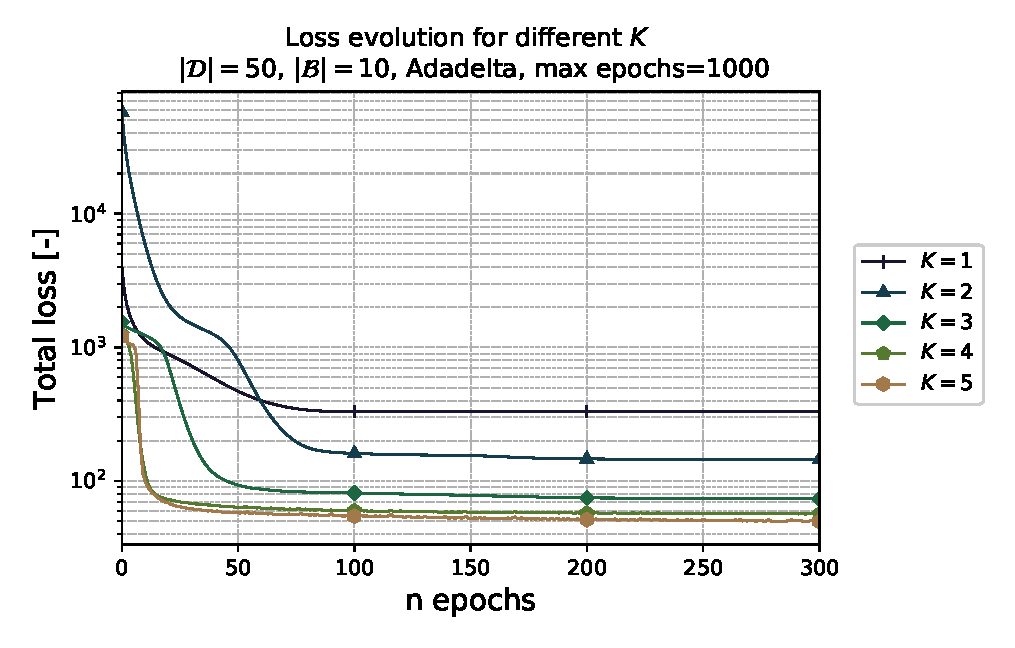
\includegraphics[width=0.8\textwidth]{figs/comparison_K.eps}
\caption{Loss evolution for different number of layers K}
\label{fig:hyperparam_K}
\end{figure}

\begin{figure}[h]
\centering
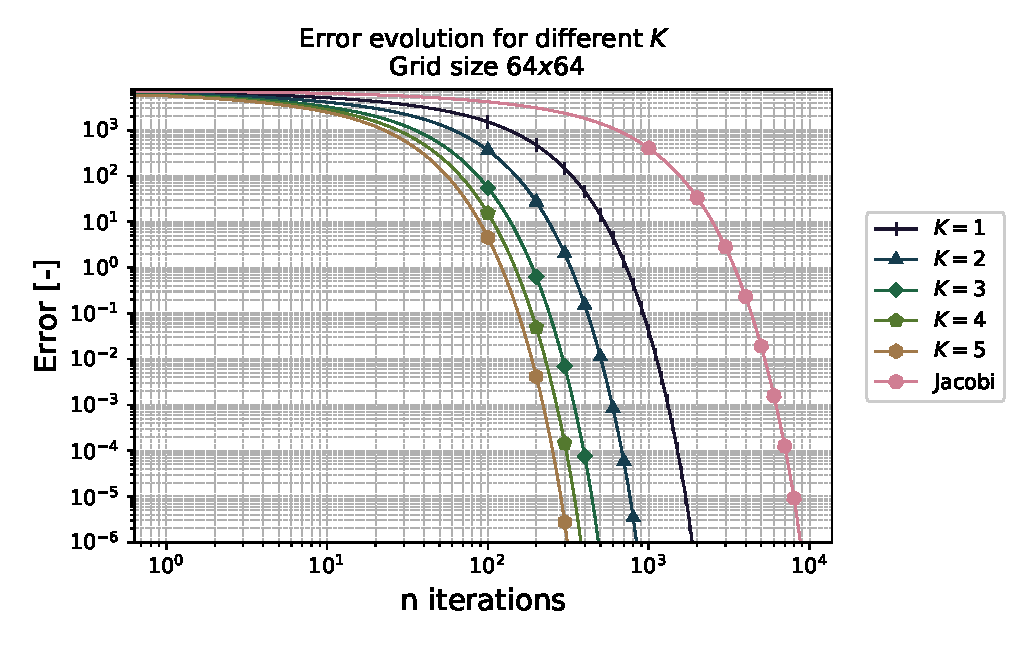
\includegraphics[width=0.8\textwidth]{figs/error_k.eps}
\caption{Error evolution w.r.t. solver iterations for different number of layers K}
\label{fig:error_K}
\end{figure}

\section{Experiments \& Results}

The hypothesis of the original paper is that a general solver can be found by training on simple domains. The simplest Laplace equation $\nabla^2u = 0$ on a square boundary shape was therefore chosen as training data.
The model was trained on $16\times16$ grid, and evaluated on grids of size $32\times32$ and $64\times64$ for both a square and an L-shaped domain. 
The L-shaped domain is created by removing a smaller square from one of the edges. Each side exhibits a different but constant boundary value chosen from a uniform distribution on the interval [-1, 1]. Thus an L-shaped domain has 6 different boundary values. The ground truth solution is obtained using the Jacobi method with a sufficient number of iterations $k=5\times10^4$. See Figure \ref{fig:example_solutions} for an example solution.

\begin{figure}[]
    \centering
    \begin{minipage}{.5\textwidth}
        \centering
        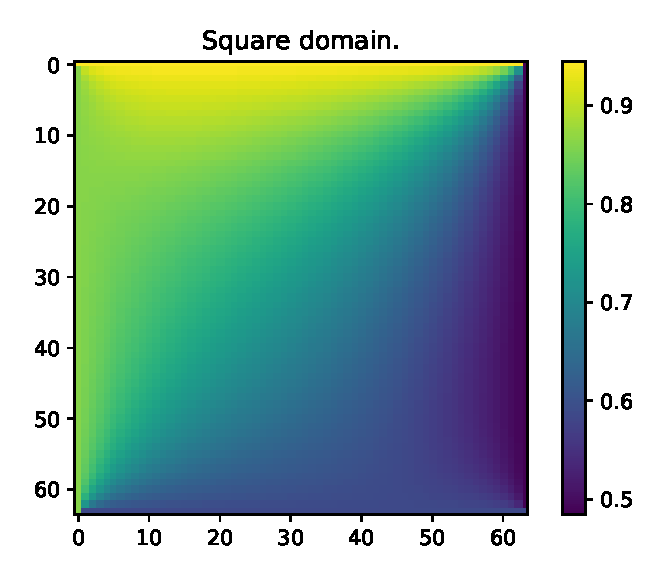
\includegraphics[width=0.8\linewidth]{figs/square.eps}
    \end{minipage}%
    \begin{minipage}{0.5\textwidth}
        \centering
        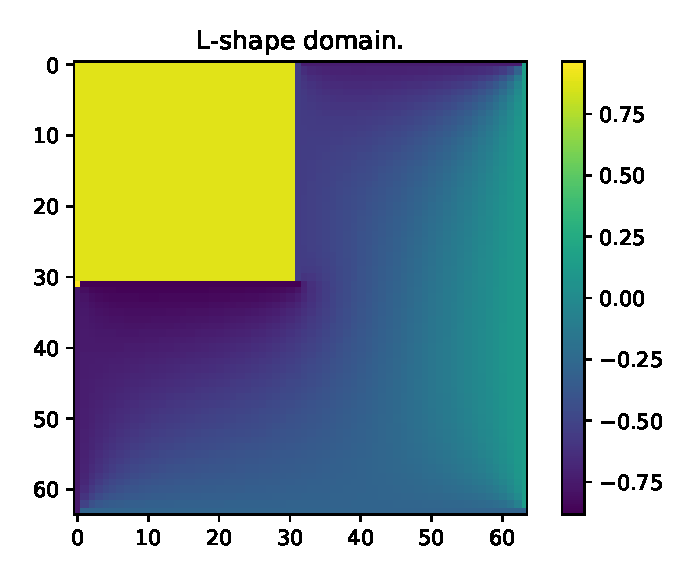
\includegraphics[width=0.8\linewidth]{figs/l_shape.eps}
    \end{minipage}
    \caption{Example solutions for the two domains.}
    \label{fig:example_solutions}
\end{figure}

In Figure \ref{fig:error_K} we shows how the error w.r.t the ground truth solution evolves with the number of iterations $k$ for the obtained solvers ($K=\{1,2,3,4,5\}$) and the Jacobi method. The learned solvers clearly outperform the Jacobi method, however we need better metrics in order to fairly compare the different models.

Both solvers were evaluated on three metrics: the number of iterations, ratio of FLOPS and ratio of CPU-time until required tolerance is reached. The number of flops were calculated assuming both solvers would be implemented using convolutional operators. This results in 4 \textit{multiply-add} operations for each element in the grid for the Jacobi iteration, whereas the learned solvers exhibit $4+9K$ \textit{multiply-add} operations. This is the same measurement as reported in the original paper, which is an estimation of the FLOPS taken. In addition to the paper we measured the CPU-time, which deemed us to be a less error-prone and more reliable measure, nevertheless both ratios gave comparable results.

As can be seen in Table \ref{tab:best_model_results} the trained solver was considerably faster than the existent solver, showing a much quicker conversion than the baseline model. Thus replicating the given results in the original paper. The highest speed-up is achieved by the 5-layer network.

%\begin{figure}[]
%    \centering
%    \begin{minipage}{.5\textwidth}
%        \centering
%        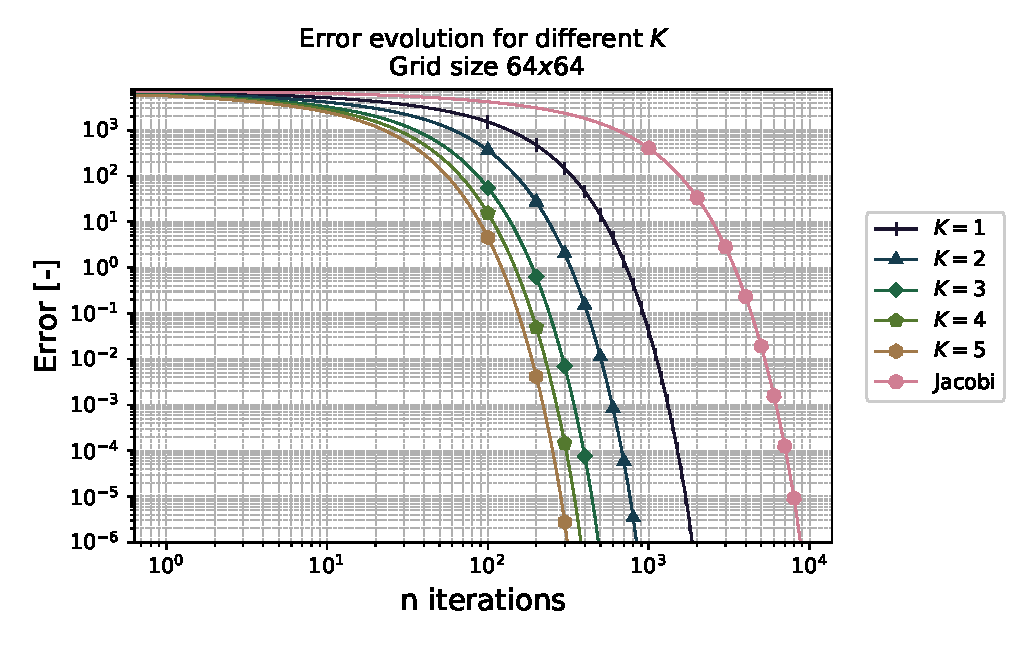
\includegraphics[width=\linewidth]{figs/error_k.eps}
%        \caption{Error evolution w.r.t. solver iterations for different number of layers K}
%        \label{fig:error_K}
%    \end{minipage}%
%    \begin{minipage}{0.5\textwidth}
%        \centering
%        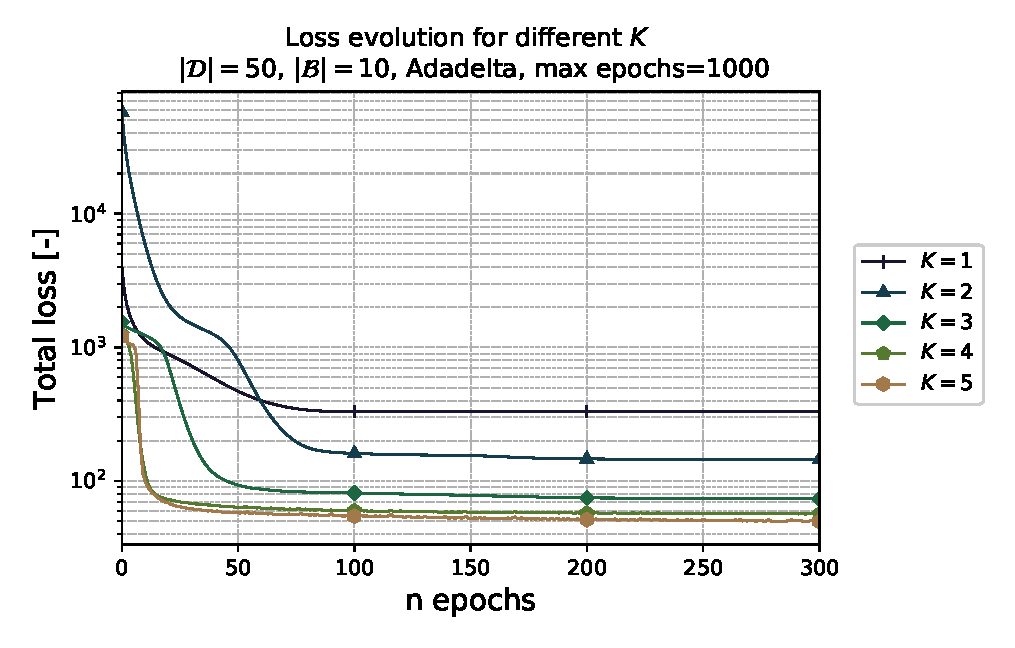
\includegraphics[width=\linewidth]{figs/comparison_K.eps}
%        \caption{Loss evolution for different number of layers K}
%        \label{fig:hyperparam_K}
%    \end{minipage}
%\end{figure}
\begin{table}[h]
    \centering
    \caption{Test results of solver trained on a $16\times16$ grid with Adadelta as optimizer. Sample size for each test of 20, number of iterations was counted until a difference to the ground truth solution of $1e-6$ or a convergence difference of $1e-12$ were achieved. Shown are the mean and the standard deviation.\\}
%\resizebox{230}{!}{
\begin{tabular}{lllccc}
\toprule
  & & & \multicolumn{3}{c}{ratios: $\frac{\text{trained solver}}{\text{existent solver}}$} \\ \cmidrule(lr){4-6}
 \thead{$K$} & \thead{Grid size} & \thead{Geometry} & \thead{FLOPS} &  \thead{CPU time [s]} &  \thead{\#iterations}$k$ \\
\midrule
\multirow{4}{*}{1} & \multirow{2}{*}{32} & l\_shape &  $0.688\pm0.001$ &  $0.308\pm0.064$ &  $0.212\pm0.000$ \\
  &    & square &  $0.688\pm0.000$ &  $0.332\pm0.097$ &  $0.212\pm0.000$ \\
\cmidrule(lr){3-6}
  & \multirow{2}{*}{64} & l\_shape &  $0.689\pm0.001$ &  $0.351\pm0.053$ &  $0.212\pm0.000$ \\
  &    & square &  $0.686\pm0.011$ &  $0.327\pm0.025$ &  $0.211\pm0.003$ \\
\cmidrule(lr){1-6}
\multirow{4}{*}{2} & \multirow{2}{*}{32} & l\_shape &  $0.518\pm0.001$ &  $0.161\pm0.032$ &  $0.094\pm0.000$ \\
  &    & square &  $0.518\pm0.001$ &  $0.171\pm0.051$ &  $0.094\pm0.000$ \\
\cmidrule(lr){2-6}
  & \multirow{2}{*}{64} & l\_shape &  $0.521\pm0.001$ &  $0.165\pm0.026$ &  $0.095\pm0.000$ \\
  &    & square &  $0.519\pm0.008$ &  $0.183\pm0.031$ &  $0.094\pm0.001$ \\
\cmidrule(lr){1-6}
\multirow{4}{*}{3} & \multirow{2}{*}{32} & l\_shape &  $0.421\pm0.001$ &  $0.106\pm0.012$ &  $0.054\pm0.000$ \\
  &    & square &  $0.421\pm0.001$ &  $0.101\pm0.013$ &  $0.054\pm0.000$ \\
\cmidrule(lr){2-6}
  & \multirow{2}{*}{64} & l\_shape &  $0.426\pm0.001$ &  $0.115\pm0.017$ &  $0.055\pm0.000$ \\
  &    & square &  $0.425\pm0.007$ &  $0.116\pm0.019$ &  $0.055\pm0.001$ \\
\cmidrule(lr){1-6}
\multirow{4}{*}{4} & \multirow{2}{*}{32} & l\_shape &  $0.401\pm0.002$ &  $0.109\pm0.028$ &  $0.040\pm0.000$ \\
  &    & square &  $0.401\pm0.002$ &  $0.095\pm0.022$ &  $0.040\pm0.000$ \\
\cmidrule(lr){2-6}
  & \multirow{2}{*}{64} & l\_shape &  $0.408\pm0.001$ &  $0.097\pm0.013$ &  $0.041\pm0.000$ \\
  &    & square &  $0.407\pm0.007$ &  $0.098\pm0.016$ &  $0.041\pm0.001$ \\
\cmidrule(lr){1-6}
\multirow{4}{*}{5} & \multirow{2}{*}{32} & l\_shape &  $0.402\pm0.002$ &  $0.078\pm0.016$ &  $0.033\pm0.000$ \\
  &    & square &  $0.402\pm0.002$ &  $0.083\pm0.016$ &  $0.033\pm0.000$ \\
\cmidrule(lr){2-6}
  & \multirow{2}{*}{64} & l\_shape &  $0.412\pm0.001$ &  $0.088\pm0.012$ &  $0.034\pm0.000$ \\
  &    & square &  $0.410\pm0.007$ &  $0.091\pm0.023$ &  $0.033\pm0.001$ \\
\bottomrule
\end{tabular}
%}
    \label{tab:best_model_results}
\end{table}

\FloatBarrier
\section{Related Work}
Recently, there have been several works on applying deep learning to solve the Poisson equation. However, to the best of our knowledge, previous works used deep networks to directly generate the solution; they have no correctness guarantees and are not generalizable to arbitrary grid sizes and
boundary conditions. This is the reason why our work was focused on reproducing the results of \cite{original_paper}, and on empirically proving the generalization of their model to arbitrary shapes and grid sizes.
\section{Conclusion \& Future work}

We could partially confirm the results reported in the original paper, not every result was reproducible either through lack of time or certainty in how these results were achieved or measured. The trained solver was able to generalize well to the presented different sizes, geometries and boundary values, while using less resources compared to the standard solver.

In the future work we would like to improve the design of the solver and the experiments in order to gain more confidence in the presented approach. For example $\mathcal{H}$ is fixed for each iteration, one could imagine a solver with different $\mathcal{H}$ for different iterations up to a certain threshold. We did not have the opportunity to test the solver using the MultiGrid method, nor the square-Poisson problem.
It is not clear how the cylinder domain was implemented in a finite difference framework, whether radial coordinates or a non uniform grid were used.

We estimate that investigating how this approach can be generalized to other type of boundary conditions other than Dirichlet or to different iterative methods such as the Gauss-Seidel method would lead to interesting results and a more applicable approach in general, as well as trying to solve different PDEs.
